\documentclass[11pt]{article}

% ── Packages ────────────────────────────────────────────────
\usepackage[margin=1in]{geometry}
\usepackage{amsmath, amssymb, amsthm}
\usepackage{booktabs}
\usepackage{graphicx}
\usepackage{hyperref}
\usepackage{natbib}
\usepackage{setspace}
\usepackage{microtype}
\usepackage{enumitem}
\usepackage{caption}
\usepackage{subcaption}
\usepackage{xcolor}
\usepackage{float}
% code packages
\usepackage{listings}
\usepackage{inconsolata}
\lstset{basicstyle=\ttfamily\footnotesize,breaklines=true}
\usepackage{csvsimple}
\usepackage{booktabs}

% ── Hyperref setup ──────────────────────────────────────────
\hypersetup{
    colorlinks = true,
    linkcolor  = black,
    citecolor  = black,
    urlcolor   = blue
}

% ── Theorem environments ────────────────────────────────────
\newtheorem{theorem}{Theorem}
\newtheorem{proposition}{Proposition}
\newtheorem{lemma}{Lemma}
\newtheorem{corollary}{Corollary}
\theoremstyle{definition}
\newtheorem{definition}{Definition}
\newtheorem{assumption}{Assumption}
\theoremstyle{remark}
\newtheorem{remark}{Remark}

% ── Spacing ─────────────────────────────────────────────────
\onehalfspacing

% ── Title block ─────────────────────────────────────────────
\title{Love of Variety Model and Simulation}
\author{Tate Mason}
\date{\today}

% ============================================================
\begin{document}
\maketitle
\thispagestyle{empty}

% ── Abstract ────────────────────────────────────────────────

\newpage
\setcounter{page}{1}

\section{Model}

\subsection{Consumer's Problem}
The consumer's problem is to maximize utility subject to their choice set. The utility function is as follows:

\begin{equation}
  U_{ijt} = \beta_i X_{jt} - (\gamma_{i}\Sigma_j)^2 + a + \xi_j + \epsilon_{ijt}
\end{equation}

\begin{gather*}
  \Sigma_j = X_{jt} - \bar{X}_{jt}
\end{gather*}

Where $U_{ijt}$ is the utility of consumer $i$ from product $j$ at time $t$. $X_{jt}$ is the attribute of product $j$ at time $t$.  $\gamma_{i}$ denotes 
a cost of sameness. $\Sigma_j$ is the sum of product attributes chosen until time $t$. Note, $\gamma_i$ has a standard normal distribution. 
$\xi_j$ captures utility from unobserved quality. Finally, $\epsilon_{ijt}$ is a  random error term distributed T1EV.

\begin{equation}
  P_{ijt} = \frac{e^{U_{ijt}}}{1 + \sum_{k} e^{U_{ikt}}}
\end{equation}

Where the denominator sums over all products $k$ in the choice set at time $t$, with the outside option.

\subsection{Firm's Problem}
The firm will maximize profits by choosing how to advertise to the consumer according to their perceptions surrounding the distribution of $\gamma$.

\begin{equation}
  \pi = (1 + a)p - c*(\kappa*a)^2
\end{equation}

Where $a$ is the advertising level and $p$ is the price of the product, $c$ is some baseline cost for the firm, and $\kappa$ is an advertising specific cost. If the firm chooses not to advertise, they get a profit of $p-c$. If they choose to advertise, they get a profit of $(1+a)p - c$.

The firm can choose to advertise at different levels, such that $a\in [0,1]$. This can be conceived of as a loss of revenue in hopes of maintaining a customer. The firm chooses $a$ to maximize profits based on the following function:

\begin{equation}
  V(a|\lambda, \Sigma_j, a_{t-1}) = \max_{\pi} \{\pi + \int_{\gamma} V'(a'|\lambda, \Sigma_j, a) d\lambda(\gamma)\}
\end{equation}

Here, $\lambda(\gamma)$ is the firm's belief about the distribution of $\gamma$ in the consumer population. $\Sigma_j$ is the sum of product attributes chosen until time $t$. $a_{t-1}$ is the advertising level at time $t-1$.
The firm chooses $a$ to maximize profits based on its current beliefs and the expected future value of advertising. Note, the distribution of $\lambda(\gamma) \sim N(\frac{1}{\Sigma_j}, \sigma_{\lambda})$.
This states they use past purchases to update their mean belief about the distribution of $\gamma$, but they have some variance in that belief.

\section{Firm Optimization}

The firm will choose $a$ to maximize profits $\pi$ based on the perceived distribution of $\gamma$ in the consumer population. The firm will also keep track of the sum of product attributes chosen by the consumer, $\Sigma_j$, to update their beliefs about $\gamma$.
The firm will solve the following optimization problem:

\begin{equation}
  V(a, \Sigma_j | \lambda(\gamma)) = \max_{a} \{\pi(a) + \int_{\gamma} V(a', \Sigma_j' | \lambda(\gamma)) d\lambda(\gamma)\}
\end{equation}

Where $\pi(a) = (1 + a)p - c*(\kappa*a)^2$ is the profit function, $\lambda(\gamma) \sim N(\frac{1}{\Sigma}, \sigma_{\lambda})$, and $\Sigma_j' = \Sigma_j + X_{jt}\cdot P_{ijt}$ is the updated sum of product attributes chosen by the consumer conditional on choosing product $j$ at time $t$.
The firm's FOC's are as follows:

\begin{gather*}
  \frac{\partial V}{\partial a} = p + P_{ijt}(1-P_{ijt})\int_{\gamma}[V(\Sigma_j + X_{jt} | \lambda'(\gamma)) - V(\Sigma_j | \lambda'(\gamma))]d\lambda(\gamma) = 0 \\
  = p + P_{ijt}(1-P_{ijt})[V(\Sigma_j + X_{jt} | \lambda(\Sigma_j + X_{jt})) - V(\Sigma_j | \lambda(\Sigma_j))] = 0 \\
  \Rightarrow p^* = (P_{ijt}(1-P_{ijt}))\cdot[V(\Sigma_j + X_{jt} | \lambda(\Sigma_j + X_{jt})) - V(\Sigma_j | \lambda(\Sigma_j))] \\
\end{gather*}

The firm will choose $a$ such that the marginal profit from advertising equals the expected marginal value of advertising in terms of future profits. The firm will update their beliefs about $\gamma$ based on the consumer's choices and the sum of product attributes chosen, $\Sigma_j$.

\section{Results}

On the consumer side, there are a few things to note. Firstly, as $\gamma$ grows, the utility becomes noisier, no matter the value of $\beta$. Secondly, notice it takes about 10 periods for utility to find some sort of stability. However, as $\beta$ grows, the time to stabilite grows.
For instance, in the low regime, it takes only five or so periods, where as in the high regime, this is closer to 20. These results suggest that $\beta$ finds a sweet spot in utility and $\gamma$ fluctuates around it.

In the firm's problem, we look at the firm's advertising decision. In the low regime, they are mostly advertising, with a couple of deviations around period 50 and 75. The rest of the regimes, however, see a lot of variation in the decision to advertise. This is to be expected,
since the firm bases its decision based off of its observations of $\Sigma$ to approximate $\gamma$. 

\clearpage

\begin{figure}
  \centering
  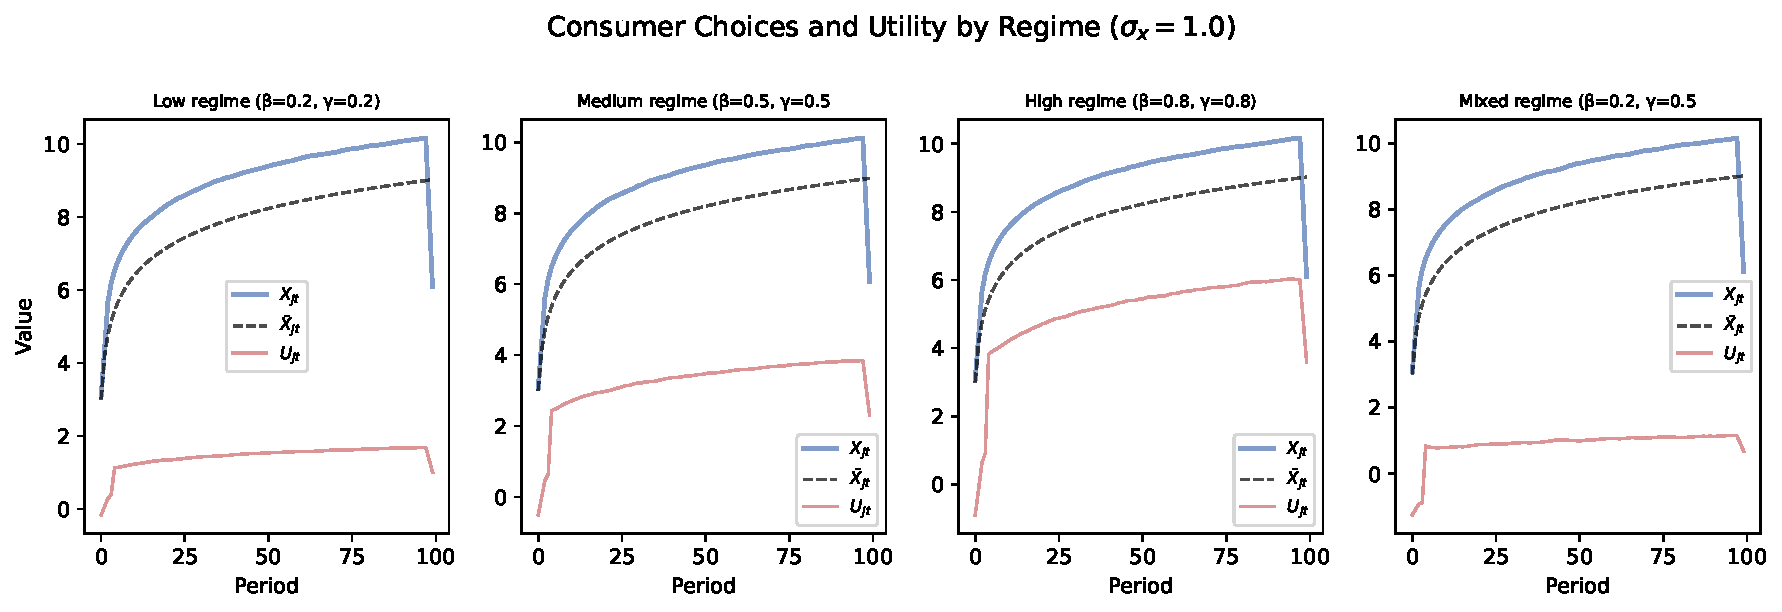
\includegraphics[width=\textwidth]{../../Output/consumer_choices_by_regime_1.pdf}
\end{figure}

\begin{figure}
  \centering
  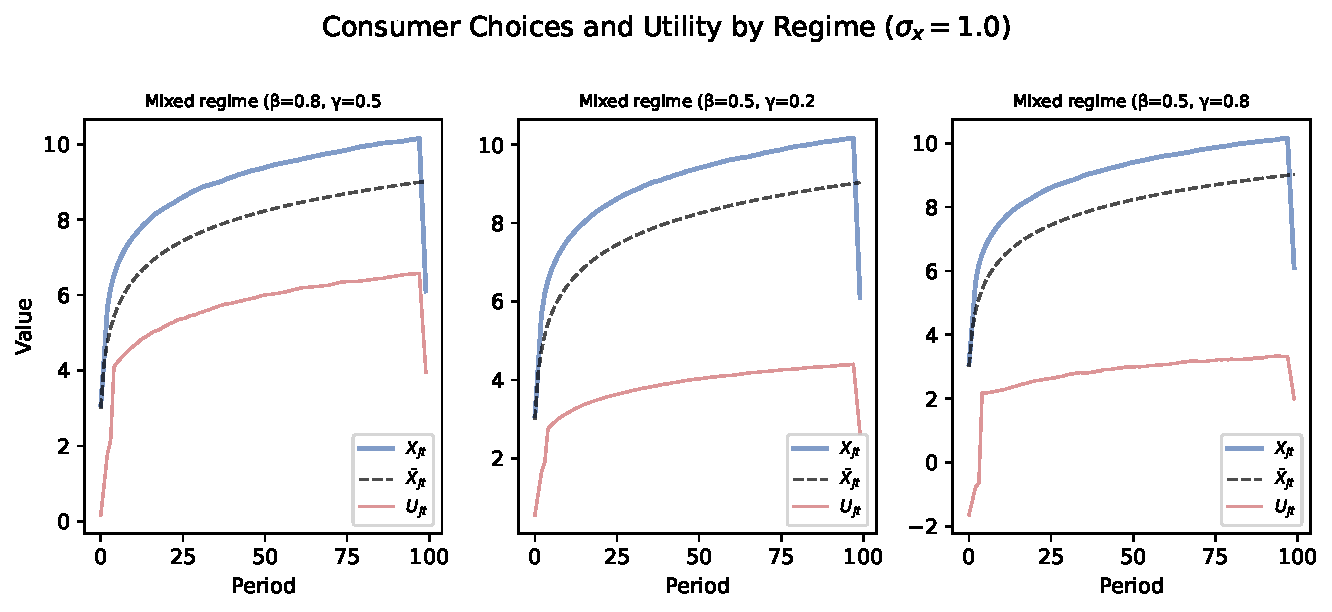
\includegraphics[width=\textwidth]{../../Output/consumer_choices_by_regime_2.pdf}
\end{figure}
\clearpage

\begin{figure}
  \centering
  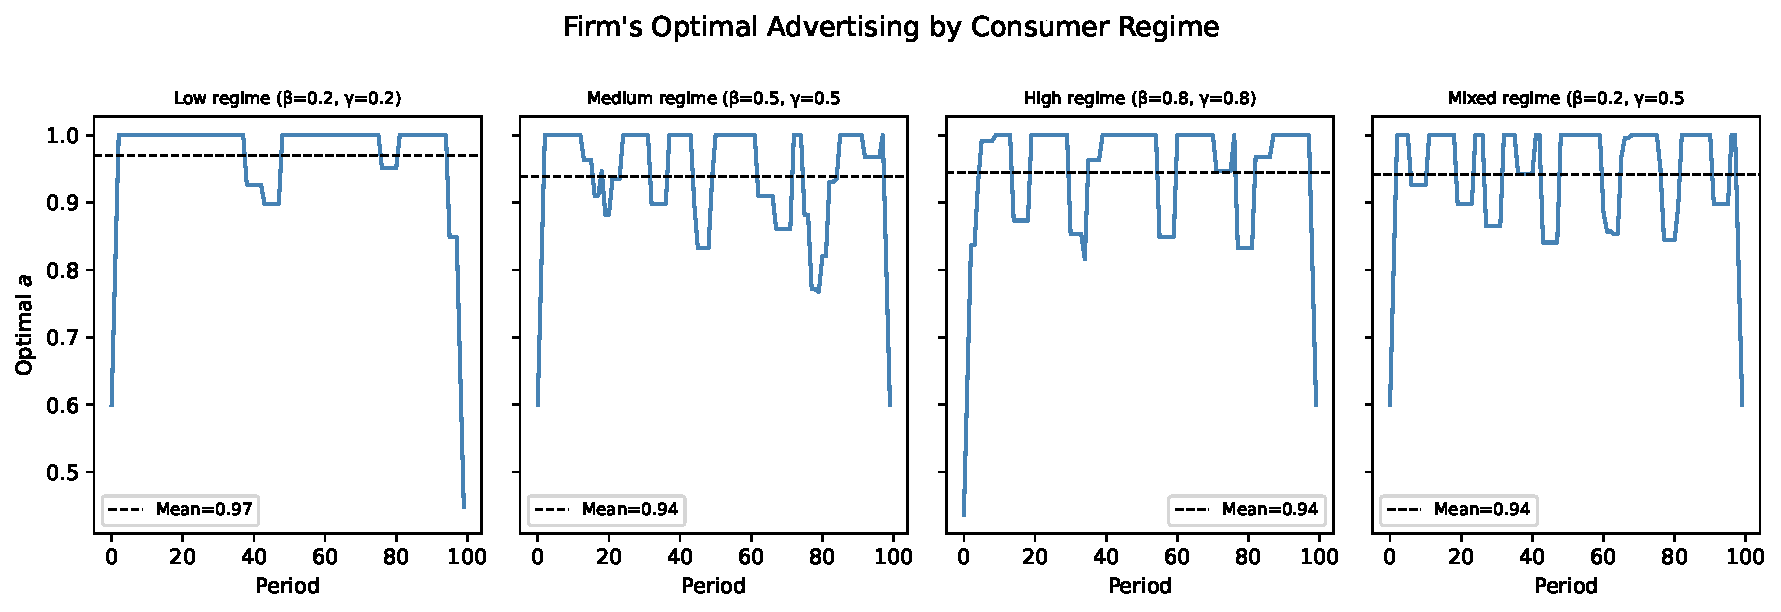
\includegraphics[width=\textwidth]{../../Output/firm_optimal_a_by_regime_1.pdf}
\end{figure}

\begin{figure}
  \centering
  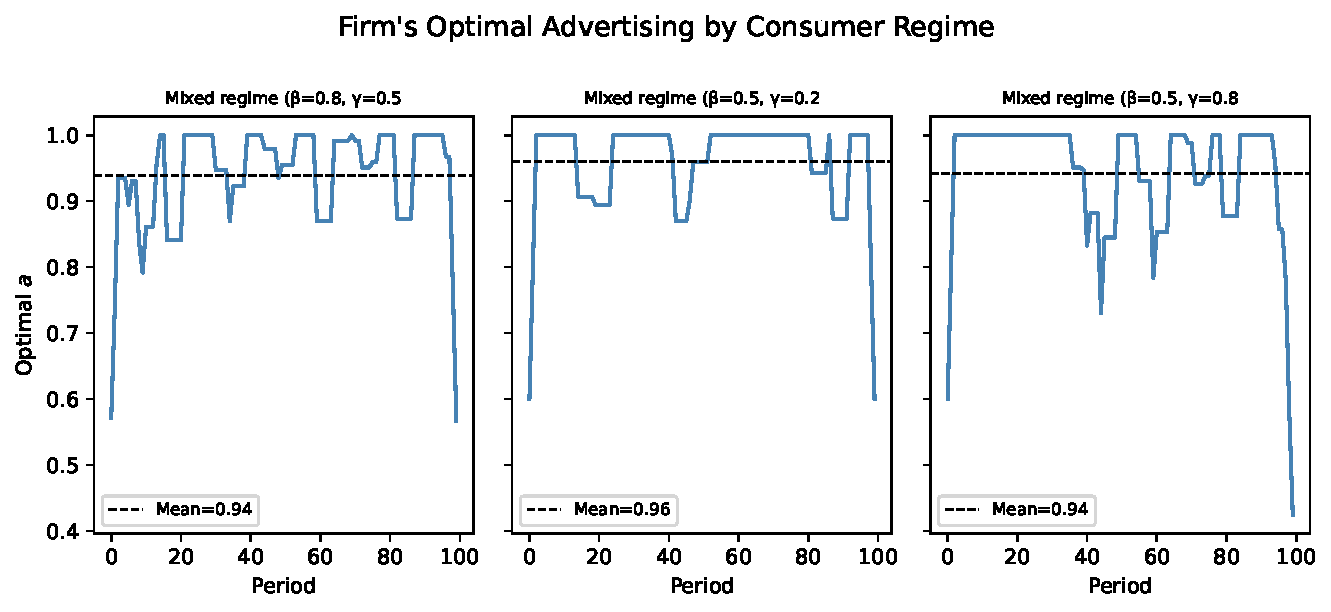
\includegraphics[width=\textwidth]{../../Output/firm_optimal_a_by_regime_2.pdf}
\end{figure}

\clearpage


\section{Code}
\lstinputlisting[language=Python]{../../Code/updated_prob.py}

\end{document}
